\documentclass{article}
\usepackage{pgfplots}
\pgfplotsset{compat=1.18}

\begin{document}

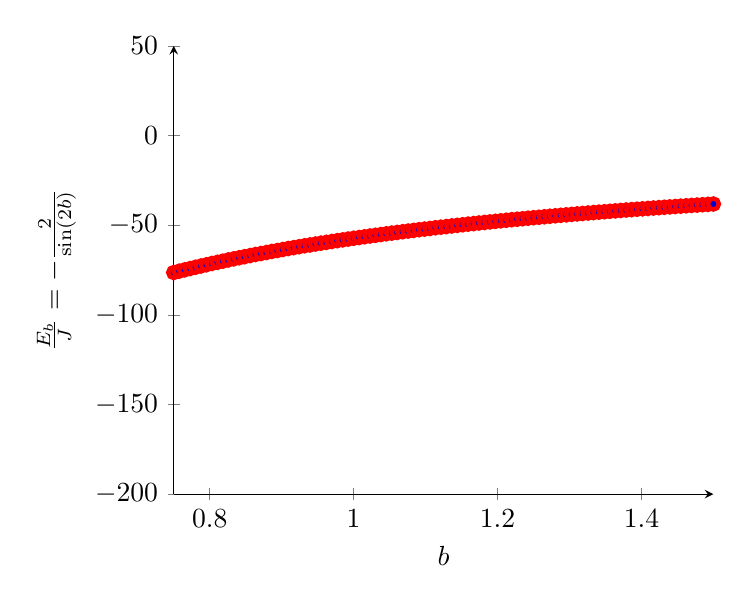
\begin{tikzpicture}
    \begin{axis}[
        axis lines = left,
        xlabel = {$b$},
        ylabel = {$\frac{E_b}{J} = -\frac{2}{\sin(2b)}$},
        ymin=-200, ymax=50,
        xmin=0.75, xmax=1.5,
        domain=0.75:1.5,
        samples=100,
        smooth,
        every axis plot post/.append style={ultra thick, red},
        ]
        \addplot {-(2/sin(2*x))};
    \end{axis}
\end{tikzpicture}

Boundary string energy as a function of \( b \) for \( \frac{\pi}{4} < b < \frac{\pi}{2} \).

\end{document}